\section{Test methodology}
\label{sec:methodology}

This test follows broadly the same principles as the one performed in September
2018.
To test the electrical continuity, a test pulse is send, and a response is read,
this time from the connectors to the readout on the flange.
\\
We perform two tests, by probing two different paths.
The first path is equivalent to the one used in September 2018
(\cref{fig:PulseCables}): a test pulse is
sent through the test pulse cables at the bottom of the anode frame, where it is
distributed typically to 32 or 256 wires (for the single termination card and
for the eight daisy chained ones, respectively).
The pulse propagates through the wires, the termination card at the top of the
anode frame, the 68 pin cables, the \DBB and finally though the interface
connector on the flange, where it is picked up by our test apparatus.
The signal path within the \DBB (\cref{fig:WireToReadout}) can be appreciated
from \cite{ICARUSDBB}, where it enters through a ``WIRE'' port
(\eg \texttt{WIRE 16\_L}) and through the
\nanoF{10} capacitor induces onto the front end (\eg \texttt{FE 16\_L}).
\\
\begin{figure}
  \subfloat[test capacitance test]{
    \label{fig:WireToReadout}
    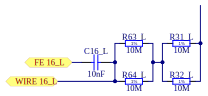
\includegraphics[width=0.48\textwidth]{fig/DBB-wire}
  }
  \subfloat[bias voltage test]{
    \label{fig:BiasVoltageToReadout}
    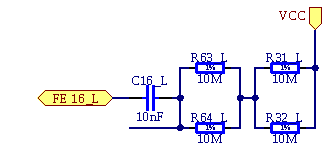
\includegraphics[width=0.48\textwidth]{fig/DBB-wire-HV}
  }
  \caption{
    DBB circuitry\cite{ICARUSDBB} involved in \protect\subref{fig:WireToReadout}
    test capacitance pulsing and \protect\subref{fig:BiasVoltageToReadout} bias
    voltage pulsing tests. The test pulse is entering through
    \protect\subref{fig:WireToReadout} ``WIRE'' and
    \protect\subref{fig:BiasVoltageToReadout} ``VCC'' port, and it is in both
    cases read out of the front-end port ``FE''.
    \label{fig:DBBcircuitryTest}
  }
\end{figure}
The second path (\cref{fig:BiasVoltageTestPath}) starts by pulsing a bias
voltage inlet.
\begin{figure}
  {
    \centering
    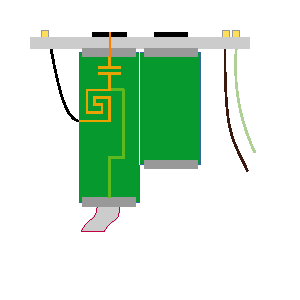
\includegraphics[height=6cm,clip,trim=0 30 0 0]{fig/BiasVoltagePath}\\
  }
  \caption{\label{fig:BiasVoltageTestPath}
    Illustration of the path of the test signal in the bias voltage connectivity
    test. The test pulse is injected through the bias voltage connector (left side),
    and follows a short path to the flange connector (represented in orange),
    bypassing the TPC wire (gray ribbon cable).
  }
\end{figure}
From there, the pulse is propagated to one side of the nine \DBB (labeled
``Cable AWG20'' in \cite{ICARUSDBB}) through the common and the channel-specific
circuitry (\cref{fig:BiasVoltageToReadout}) before reaching the front-end
readout.
It should be noted that the bias voltage circuitry is designed for a constant,
large voltage (\V{300}), while the test pulse is small (a few volt) and rapidly
changing.
Therefore, features observed in this test may be not significant for the regular
operation of the detector.
\\
These two paths test different paths of the circuitry
(\cref{fig:DBBcircuitryTest}).
The first path (\cref{fig:WireToReadout}), pulsing the wire through the test
capacitance, tests the full signal path, and barely grazes the \DBB circuitry.
The second one (\cref{fig:BiasVoltageToReadout}) instead skips the wire but goes
through most of the \DBB components.
The flanges had gone through a specific test for bias voltage distribution, that
test is not sensitive enough to pin down a failure on a single channel.
Also, as will be described in the result section (\cref{sec:results}), having a
test including the wire and one excluding it allowed to pin down very precisely
a faulty installation where a 68 pin cable was not correctly connected.
\\
Both the paths we use for testing are necessarily \emph{discontinuous}: both
include a \nanoF{10} capacitor on the \DBB just in front of the front end
outlet, and in addition the wire path also includes an uncalibrated,
picofarad-level capacitance on the bottom termination card.
As a consequence, the test can't directly verify the continuity of the paths,
and we rather have to interpret its response.
\\
The bias voltage path bypasses the wire altogether, and it is therefore the same
for all flanges on all chimneys, including the ones serving the first induction
plane.
In addition, for a few flanges the test on the bias voltage path was performed
also before the flange being mounted on the detector.
That configuration is effectively almost identical to the one on the detector,
with the exception that the wire is not connected at all and, for example, does
not contribute to pick up noise.
\\
To test the first induction plane wires, a modified test was devised: because
those wires lack a test capacitance, signal is induced on them from the wires
\emph{on one of the other planes}. This results in the path shown in
\cref{fig:WireToReadoutInduced}. The pulse is injected into a chimney on the
same column, chosen to maximize the overlap of the pulsed wires with the ones
to be tested. To have the large signal possible, the pulse cables are chosen
which are connected to eight daisy-chained test capacitance cards.
This path is effectively equivalent to adding a capacitance in series to the
test capacitance, this one made of air dielectric and wired arms.
As a rough idea of the configuration, each first induction plane wire can be
considered an arm \mm{3} wide, and as long as \cm{\approx 90} (that is, the
space covered by the 256 pulsed wires: $8 \times \mm{11}$ of each card), far
\mm{3} from the other arm. The chimney chosen to be pulsed was always 5 chimneys
away from the end, that is chimneys \texttt{06} and \texttt{15}, close to the
middle of the fist induction plane. No difference was observed in the signal
induced by pulsing one plane or the other of that chimney, despite one of them
being twice as far as the other.
\begin{figure}
  {
    \centering
    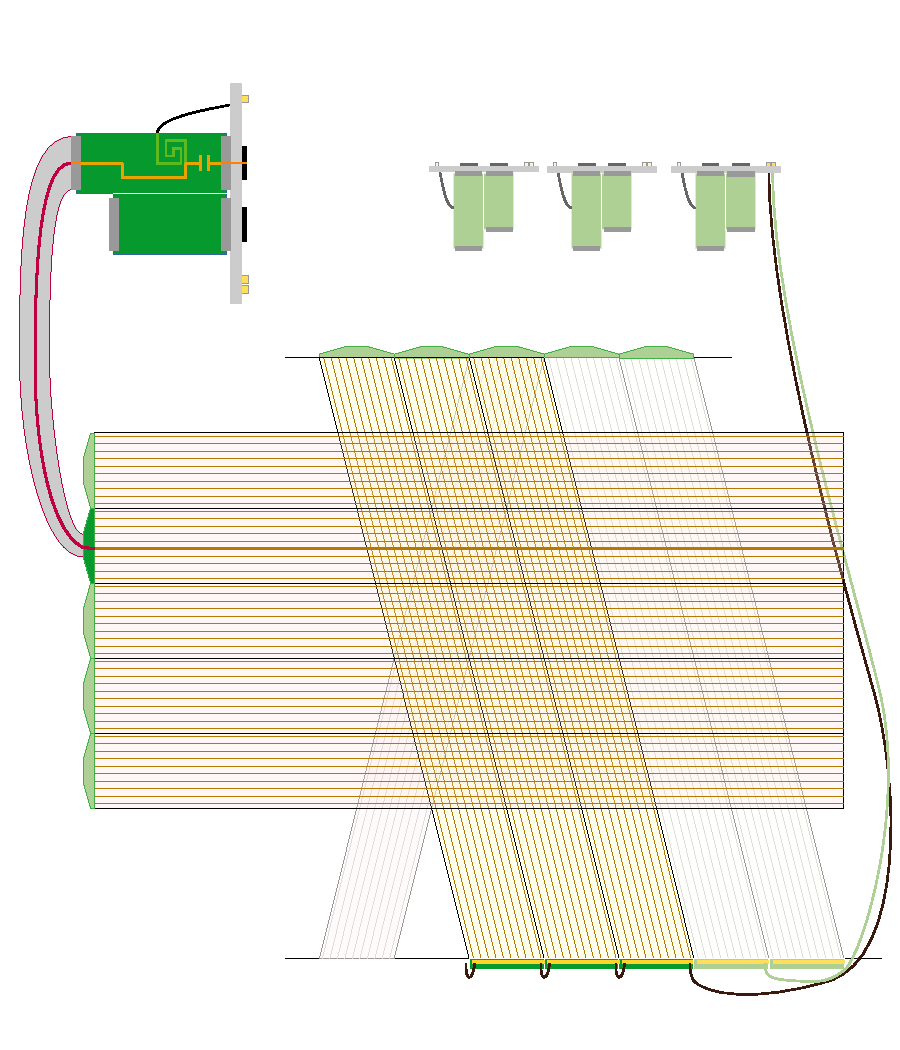
\includegraphics[height=6cm,clip,trim=0 30 0 0]{fig/PulseCableHorizontalPath}\\
  }
  \caption{\label{fig:WireToReadoutInduced}
    Illustration of the path of the test signal for the first induction plane
    wires.
  }
\end{figure}
It should be noted that in this configuration all the 1056 wires of the half
plane are pulsed at the same time. This increases the amount of cross talk
between the 68-wire cables.
\\
No connectivity test was performed on the $\approx 4000$ short wires shown in
\cref{fig:WireCategories} as red category.


\subsection{Test setup}
\label{ssec:methodology:setup}

The test pulse is generated with a ``test box'' designed by Mark Convery
(\cref{fig:TestBox}), which includes a pulse generator and also provides
amplification of the response to the pulse.
After amplification, the responses are digitized by a four-channel oscilloscope
(\href{https://www.tek.com/datasheet/digital-phosphor-oscilloscopes-0}{Tektronix TDS 3054C})
and sent to a program running on a laptop, which can record them as waveforms
(\cref{fig:TestSetup}).
The path followed by the test pulse is illustrated in the following paragraphs.
\\
\begin{figure}
  {
    \centering
    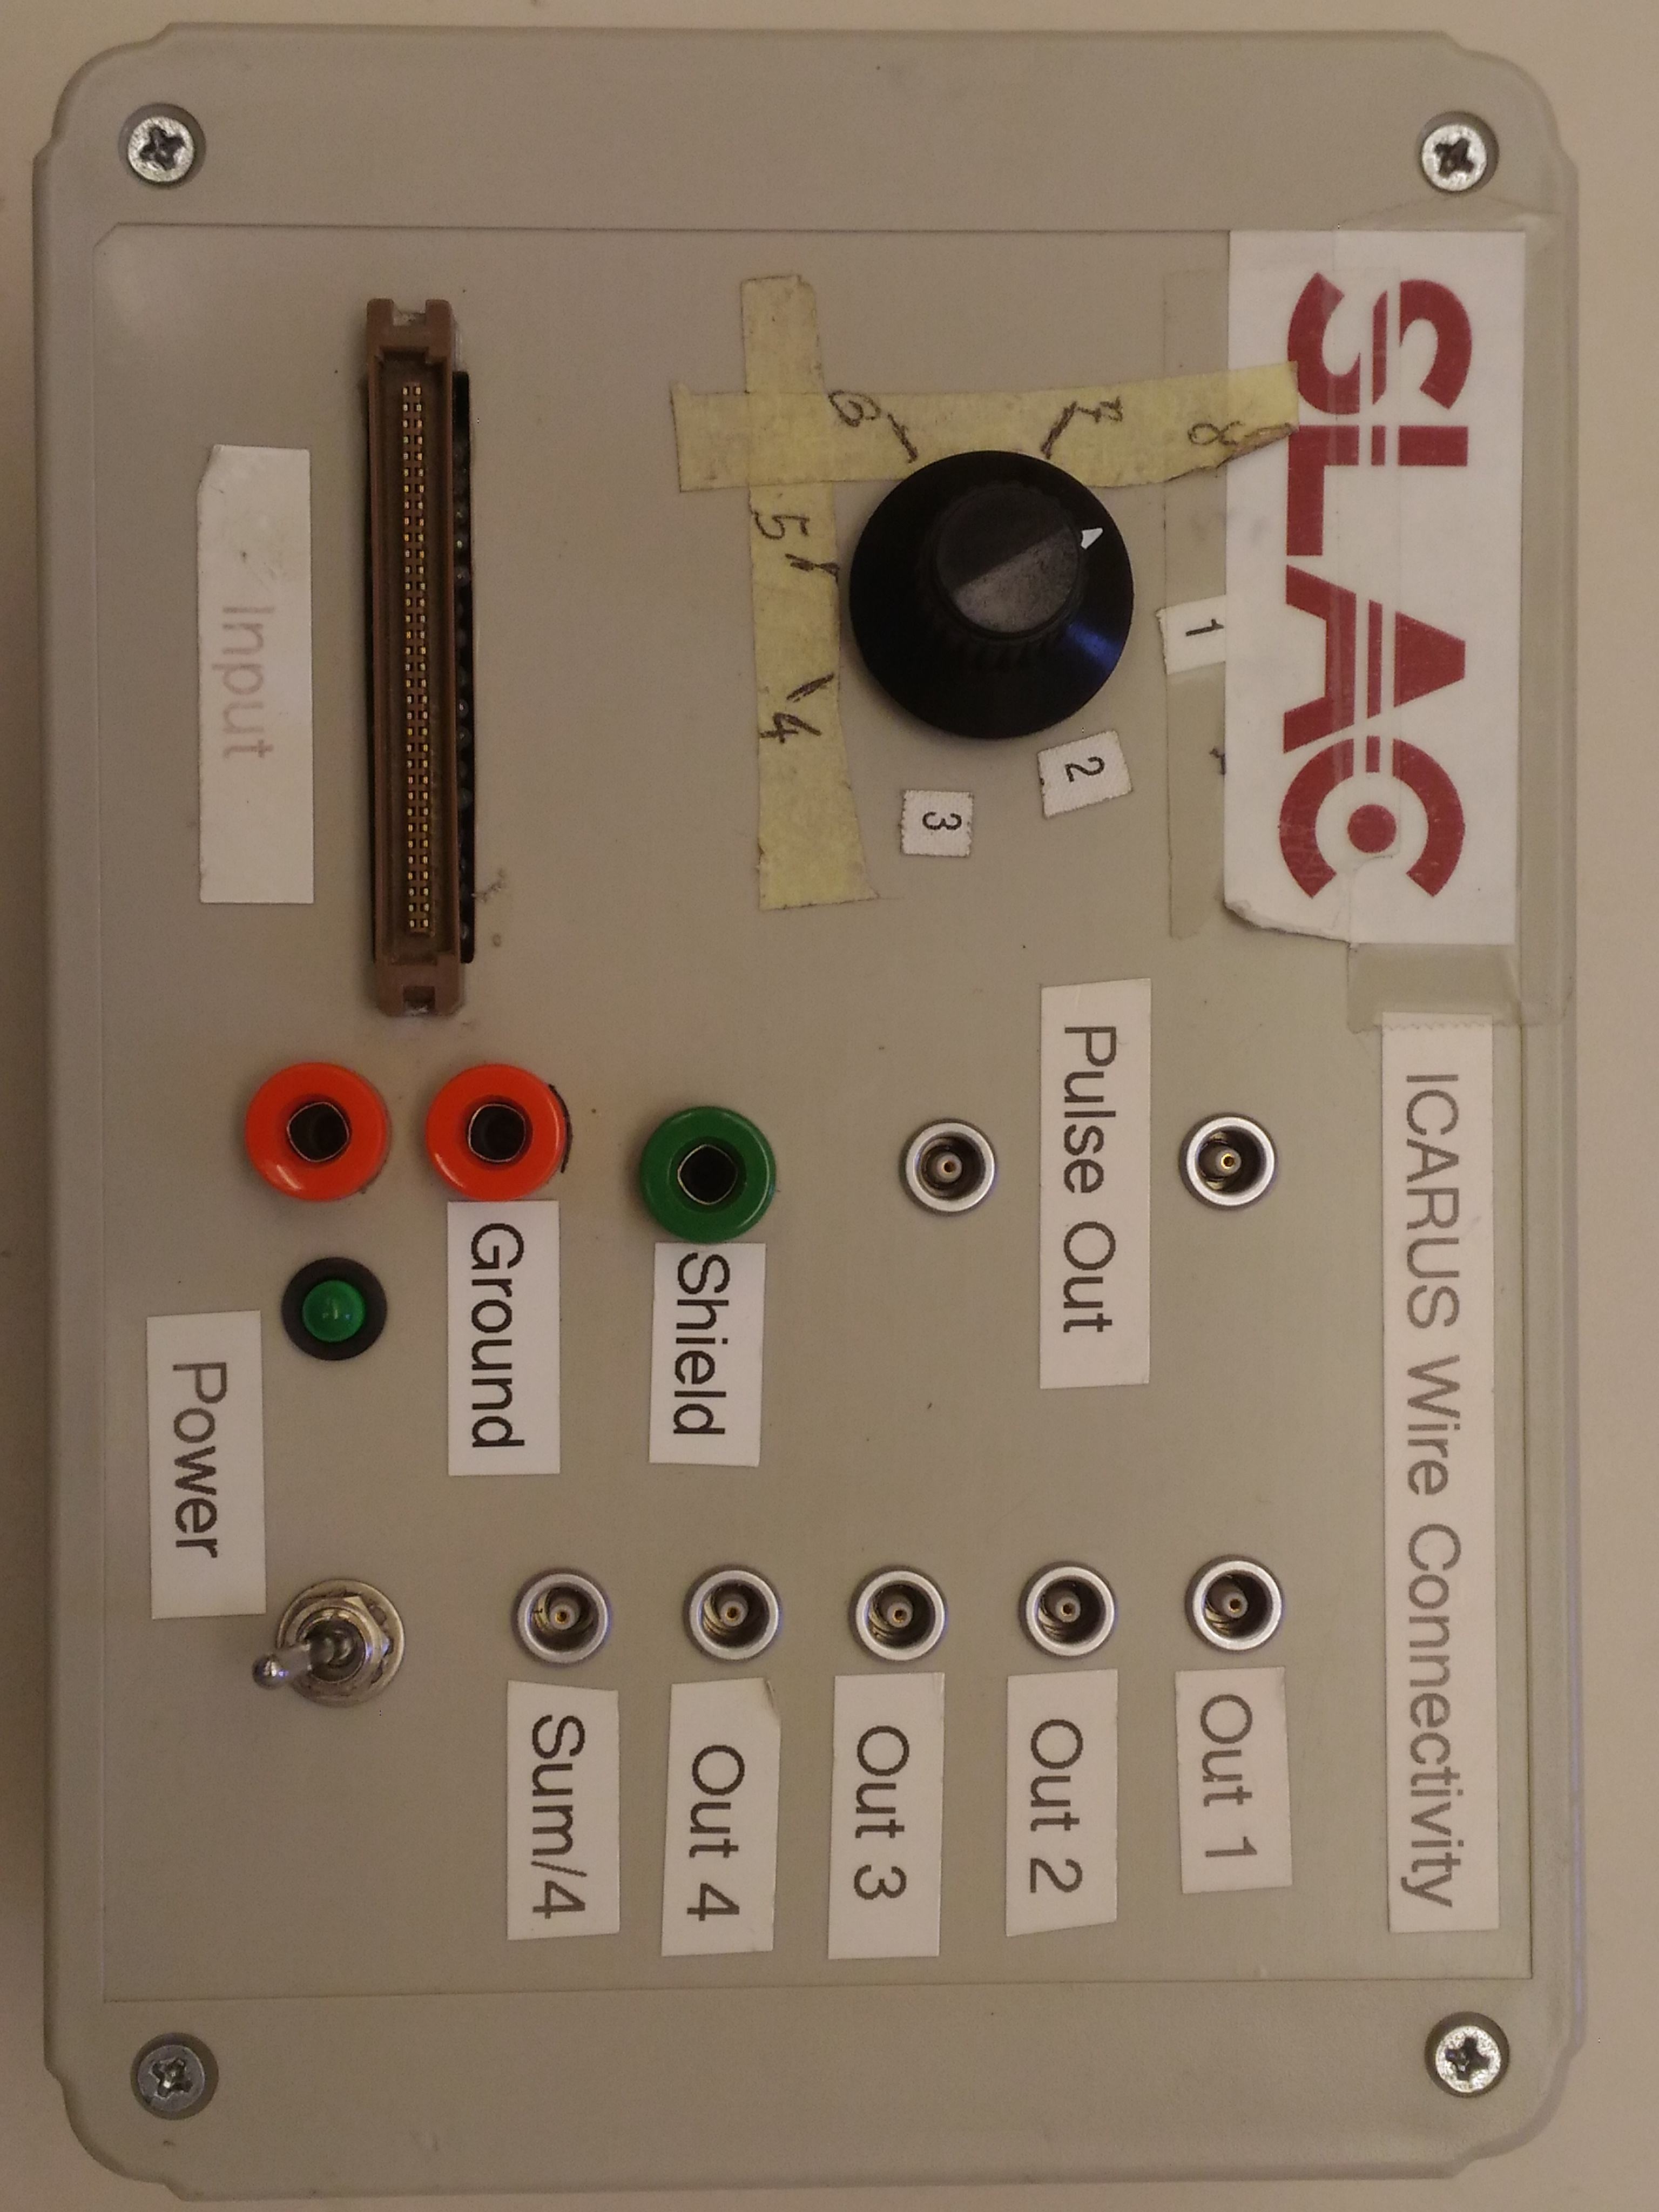
\includegraphics[height=6cm]{fig/20190501_113323-TestBox}\\
  }
  \caption{\label{fig:TestBox}
    The older one of the the two test boxes used for generating the test pulse
    and selecting and amplifying the response to it.
  }
\end{figure}
\begin{figure}
  % there should be somewhere an illustration of the setup...
  \qquad
  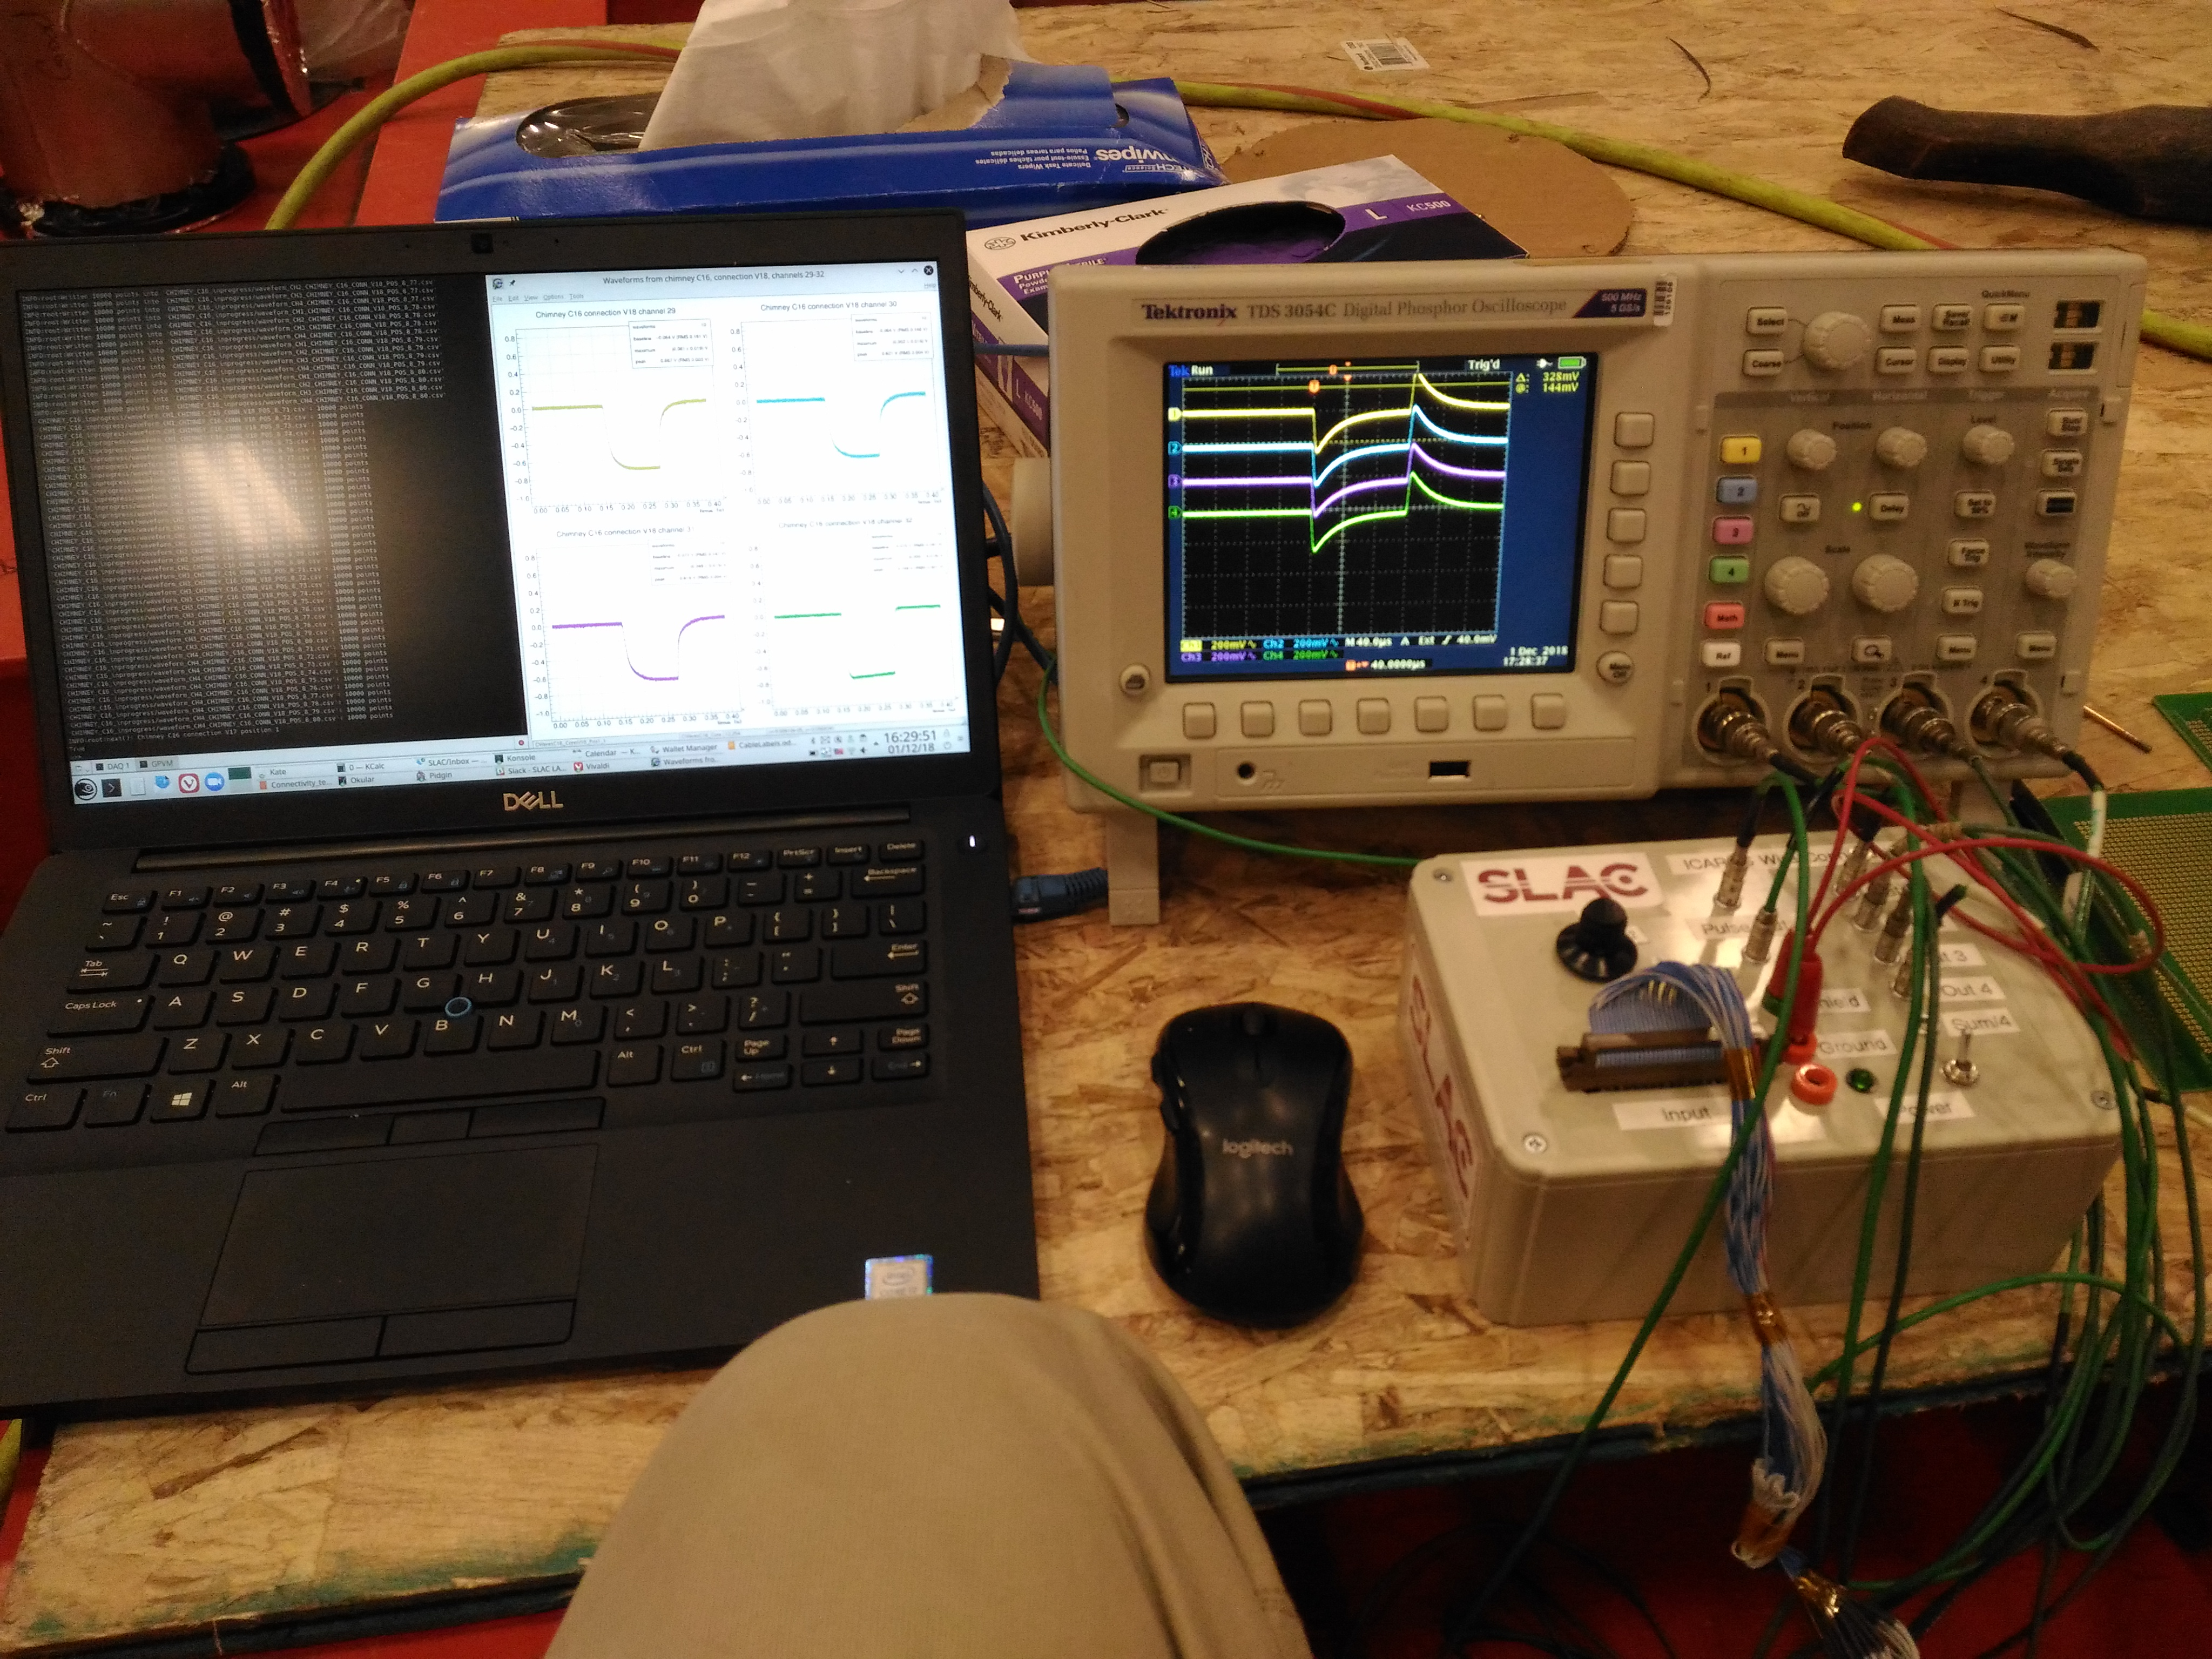
\includegraphics[width=0.48\textwidth]{fig/2018-12-01_16-29-52-ConnectivityTestReadoutSetup}
  \caption{\label{fig:TestSetup}
    Connectivity test readout setup.
  }
\end{figure}
The test boxes are the same used in the testing of September 2018, including the
dead channels (channel 2 in one of the boxes, channel 18 in the other), with
some upgrade.
The boxes are powered by three \V{1.5} AA batteries, and they now include a
voltage regulator that stabilizes the output at about \V{3.3}.
The test pulses are emitted at a rate of \Hz{100}, each one a positive square
wave of \V{3.3} with a duration of about \micros{100}.
\begin{figure}
  \subfloat{
    \raisebox{-0.5\height}{
      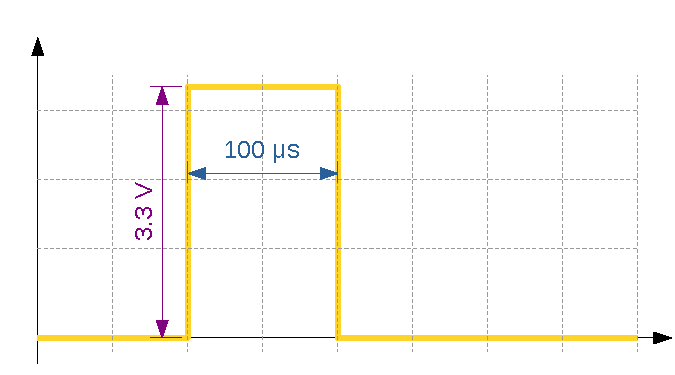
\includegraphics[width=0.48\textwidth]{fig/TestPulseCartoon}
    }
  }
  \subfloat{
    \begin{tabularx}{0.4\linewidth}{ll}
      \hline
      shape          & square wave         \\
      amplitude      & \V{3.3}             \\
      length         & \micros{\approx100} \\
      pulse rate     & \Hz{100}            \\
      \hline
    \end{tabularx}
  }
  \caption{
    Illustration and specifications of the pulse used in connectivity tests.
  }
  \label{fig:TestPulse} 
\end{figure}
Each test box includes two outlets for the same pulse.
One is sent directly to the oscilloscope to work as a trigger.
The other is sent to the detector via a lemo to SMA cable: it will be plugged
either to the test pulse cable or to the bias voltage distribution, to implement
one of the two test paths described in \cref{sec:methodology}.
The response to these pulses is read from the front end connectors on the
flange.
The standard setup includes the installation of an empty readout minicrate, its
only purpose to provide mechanical support, and in it a board shaped as a
readout board, which is in effect just a passive adapter from the front end
connector to a 68 pin cable: each of these ``fake'' readout boards includes two
such adapters, converting at once both the left and the right side connectors,
and allowing for two different 68 pin cables.
At a time, the correct one of the two cables (for example, the left one when the
test is currently pulsing the left bias voltage distribution path) is plugged
back into the test box, conveying signals from the 32 channels from the \DBB
side it is connected to.
The test box contains a eight position switch that selects four contiguous
channels among the 32 from the cable.
Signals from the four channels are amplified and offered each on an independent
outlet.
These four channels are sent to the oscilloscope for digitization and visual
inspection.
The oscilloscope can be driven by commands sent via Ethernet from a laptop,
where a simple data acquisition program drives the readout and recording of the
digitized waveforms.
One of the test boxes also offers ``direct'', non-amplified versions of the
signal.
\\
Noise and grounding have been an issue in the previous session of tests.
Depending on the grounding of the shield wires, they do actually act as shield,
or they rather act as antennas picking up noise.
The upgraded test boxes allow the option of connecting all the shield wires to
the ground (which is effectively the oscilloscope ground).
This option was regularly used in the December 2018 testing session.
It results into reduced noise and also in reduced signal response, allegedly
because of reduction of cross talk from other cables.
In addition, we grounded the oscilloscope chassis to the detector.


\subsection{Data acquisition}
\label{ssec:operations:DAQ}

The Tektronix TDS 3054C oscilloscope can digitize and send out the input
signals, providing $10^4$ samples per channel,
each sample with 8-bit precision\footnote{
The oscilloscope alternatively allows for 9 bit ADC conversion, at the cost of
doubling the data size}.
The custom data acquisition code reads a sequence of waveforms from each
oscilloscope channel.
Each waveform is stored in its own comma-separated value file (CSV),
with a resolution of \micros{0.1} for the time and \milliV{10} for the signal
amplitude. Therefore the waveform samples span 1 millisecond, and they are at
baseline in roughly $60-80\%$ of the time.
\\
The testing procedure included cycling across all 8 switch positions of the test
box for each connection, and recording 10 waveforms for each of the 4 channels
monitored in the selected position. For each switch position, therefore,
40 waveforms are recorded. The total data size as stored in the final form is
about \mebiB{500} per chimney.


\subsection{Labelling}
\label{ssec:labelling}

\begin{figure}
  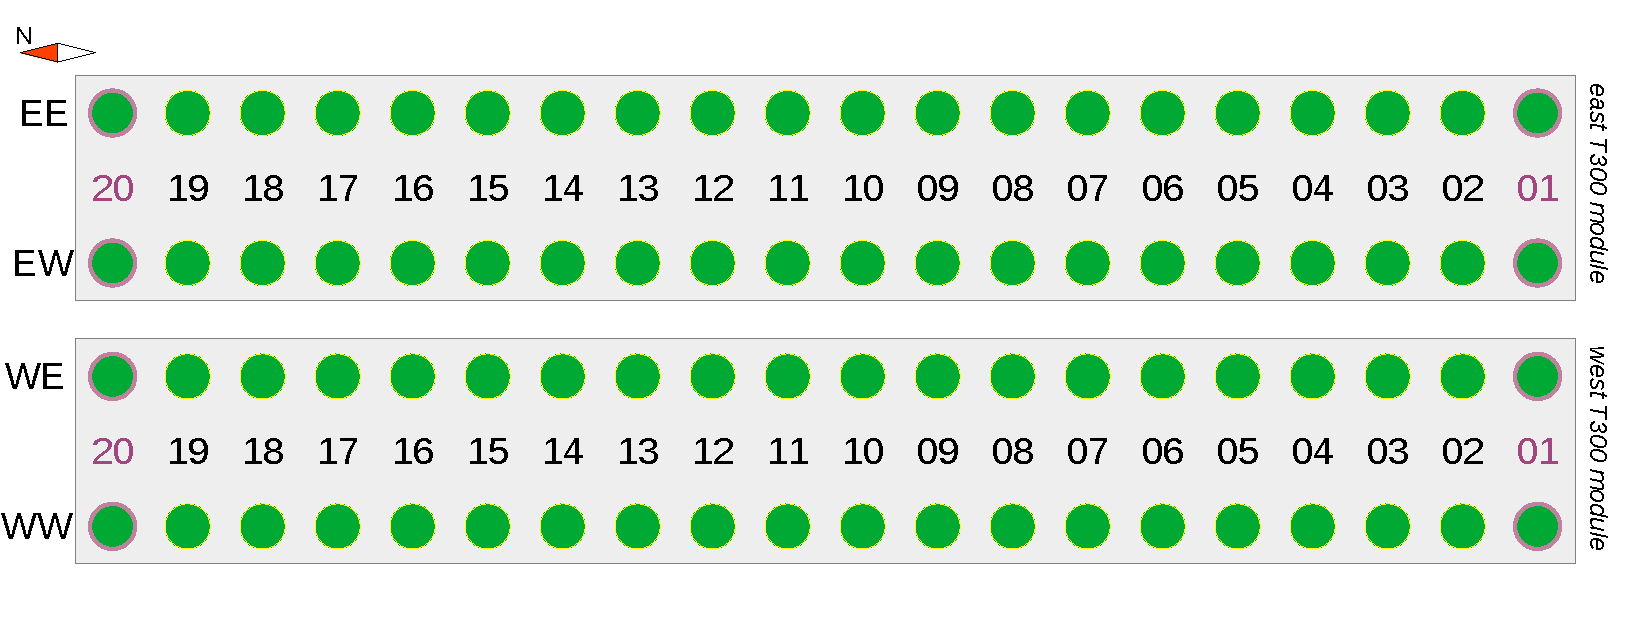
\includegraphics[width=\textwidth,clip,trim=0 35 0 10]{fig/ChimneyMap}
  \caption{\label{fig:ChimneyLabelling}
    Disposition and labeling of the chimneys. End chimneys (\texttt{01} and
    \texttt{20}) are circled in magenta.
  }
\end{figure}

We use the following labeling conventions:
\begin{description}
  \item[chimneys] are laid out in four ``columns'' and twenty ``rows'':
    \begin{itemize}
      \item columns are labeled geographically, with the position of the module
            first (\texttt{E}ast or \texttt{W}est) and then the side within the
            module (also \texttt{E}ast or \texttt{W}est)
      \item rows are numbered \texttt{01} (the most northern one) to \texttt{20}
            (the most southern one, the side neutrino beams come from)
    \end{itemize}
    Chimneys \texttt{01} and \texttt{20} are taller and host three flanges,
    and they have been called ``end'', ``corner'', or ``tall'' chimneys;
  \item[flanges] are rarely referred to directly; we'll use the letter
    \texttt{F} followed by the flange number, that effectively went from 1 to
    100 (there are 96 flanges mounted on the detector, but spares were produced
    as well)
  \item[cables] (68-wire cables) are numbered from \texttt{01} to \texttt{18},
    except for the ones serving the first induction plane, where the range
    extends to \texttt{33}; the cables have a letter tag too, which can be
    \texttt{V} (east side of each module), \texttt{S} (west side of each
    module), or \texttt{A}/\texttt{B}/... in the end chimneys; since this cable
    tag does not add any information, occasional inconsistencies are
    nonconsequential
  \item[channels] and wires are usually identified by a number between 1 and 32
    within each cable, with channel 1 being the one marked by the red wire on
    the cable itself. In connectivity test context, a 4-channel oscilloscope
    is used for digitization, and a channel $c$ might be designed by test box
    switch position ($p$) and oscilloscope channel ($CH$) instead: the numerical
    rule is $ c = 1 + 4 (p - 1) + (CH - 1) $
  \item[position] of the switch in the test box spans the range 1--8, where
    position 1 covers channels 1 to 4, position 2 covers channels 5 to 8, up to
    position 8 covering channels 29 to 32
  \item[oscilloscope channel] is one of the four channels of the oscilloscope;
    we use to color-code them as yellow (CH1), cyan (CH2), green (CH3) and
    magenta (CH4), after the color the oscilloscope associates them to. In
    general it is recommended that the channel as defined above is used instead,
    which is not bound to this specific test.
\end{description}


